\documentclass[journal,article,submit,pdftex,moreauthors]{Definitions/mdpi} 
\usepackage{changepage}
\usepackage{graphicx} 
\usepackage{caption}  


\Title{Aplikasi SafeSpeak Untuk Mendeteksi Komentar Negatif}

\TitleCitation{Aplikasi SafeSpeak Untuk Mendeteksi Komentar Negatif}

\newcommand{\orcidauthorA}{0000-0000-0000-000X}

% Authors, for the paper (add full first names)
\Author{Laode Fahmi Hidayat $^{1,\dagger,\ddagger}$\orcidA{}, Muhammad Iswari $^{2,\ddagger} $ Muh Azka Sufirman Rahman $^{3,\ddagger}$ Andi Adnan $^{4,\ddagger} $ Ayu Widianti $^{5,\ddagger} and  $ Rezqia Nurqalbi $^{6}$}

\AuthorNames{Laode Fahmi Hidayat, Muhammad Iswari, Muh Azka Sufirman Rahman, Andi Adnan, Ayu Widianti, Rezqia Nurqalbi}

\AuthorCitation{Hidayat; Iswari; Rahman; Adnan; Widianti; Nurqalbi;}

\address{%
$^{1}$ \quad Universitas Hasanuddin ; iswarihasis@gmail.com \\
$^{2}$ \quad Universitas Hasanuddin ; azkasufirman3@gmail.com \\
$^{3}$ \quad Universitas Hasanuddin; bayubulan659@gmail.com  \\
$^{4}$ \quad Universitas Hasanuddin ; adnanandi252@gmail.com  \\
$^{5}$ \quad Universitas Hasanuddin ; ayuwdnti13@gmail.com \\
$^{6}$ \quad Universitas Hasanuddin ; rezqianurqalbi8@gmail.com }

% \corres{Correspondence: e-mail@e-mail.com; Tel.: +xx-xxxx-xxx-xxxx (F.L.)}

\begin{document}

\section{Materials and Methods}

\subsection {IndoBert}

\begin{adjustwidth}{2em}{0pt} 
\hspace{0.3cm} BERT (Bidirectional Encoder Representations from Transformers) adalah model pembelajaran mendalam berbasis Transformer yang dikembangkan oleh Google. BERT dirancang untuk memahami konteks linguistik secara lebih mendalam dengan memproses teks dalam dua arah (bidirectional), yaitu dari kiri ke kanan dan dari kanan ke kiri secara bersamaan. Dengan pendekatan ini, BERT dapat menangkap hubungan antar kata dalam sebuah kalimat atau dokumen secara lebih komprehensif, termasuk konteks makna kata berdasarkan posisi dan penggunaannya dalam kalimat. Model ini dilatih menggunakan dua teknik utama yaitu masked language modeling (MLM) dan next sentence prediction (NSP), yang memungkinkannya menangkap semantik dan sintaksis secara mendalam.

IndoBERT adalah adaptasi BERT untuk bahasa Indonesia. Bahasa Indonesia memiliki karakteristik linguistik yang unik, sehingga penggunaan model BERT standar sering kali kurang optimal. IndoBERT dilatih secara khusus pada kumpulan data besar yang mencakup berbagai variasi teks dalam bahasa Indonesia, sehingga mampu memahami konteks, tata bahasa, dan makna dalam bahasa Indonesia dengan lebih baik. Dengan demikian, IndoBERT menjadi solusi yang lebih relevan untuk berbagai aplikasi pemrosesan bahasa alami (NLP) dalam bahasa Indonesia, seperti klasifikasi teks, analisis sentimen, dan penerjemahan otomatis.

IndoBERT dalam aplikasi SafeSpeak berfungsi sebagai model untuk mendeteksi komentar negatif secara otomatis. SafeSpeak menggunakan IndoBERT untuk menganalisis teks komentar yang diterima. Proses ini dimulai dengan tokenisasi, di mana teks dibagi menjadi unit-unit yang dapat dipahami oleh model. Setelah itu, IndoBERT menentukan sentimen dari komentar tersebut, apakah positif atau negatif.
\end{adjustwidth}

\item \hspace{1cm} 1.1.1 Langkah - Langkah IndoBert
\begin{adjustwidth}{4em}{0pt} 
\begin{itemize}
    \item \textbf{Pre-training :} 
    Pada tahap pertama, IndoBERT dilatih menggunakan dataset berbahasa Indonesia yang bersumber dari Kaggle. Tujuan dari pra-pelatihan ini adalah agar IndoBERT dapat memahami pola bahasa Indonesia, struktur kalimat, dan hubungan antar kata, sehingga model ini mampu mengenali konteks dalam bahasa Indonesia, baik dalam bentuk bahasa formal maupun informal.
    \item \textbf{Fine-Tuning :} 
    Setelah melalui pra-pelatihan, IndoBERT dilakukan fine-tuning untuk tugas tertentu, yaitu deteksi sentimen negatif dalam komentar. Pada tahap ini, model dilatih menggunakan dataset yang telah diklasifikasikan berdasarkan sentimen (positif, negatif, dan netral). Fine-tuning ini memastikan IndoBERT dapat mengenali emosi atau nada dalam komentar dan mengidentifikasi sentimen negatif dengan lebih akurat.
    \item \textbf{Tokenisasi Teks :} 
    Setelah fine-tuning, IndoBERT siap digunakan dalam aplikasi. Ketika sebuah komentar baru diterima, teks komentar tersebut akan melalui proses tokenisasi, di mana teks dipecah menjadi unit-unit kata atau token yang dapat dipahami oleh model. Tokenisasi ini memungkinkan IndoBERT untuk memproses kalimat dengan lebih efisien.
    \item \textbf{Analisis Sentimen dengan IndoBERT :} 
    IndoBERT menganalisis teks untuk menentukan sentimen dari komentar tersebut. Model ini menghitung probabilitas sentimen yang terkandung dalam komentar dan memutuskan apakah komentar tersebut mengandung sentimen positif atau negatif.
    \item \textbf{Penyempurnaan dan Pembaruan :} 
    IndoBERT terus disempurnakan dengan memperbarui dataset dan melakukan fine-tuning lebih lanjut berdasarkan feedback dan data terbaru. Dengan pembaruan ini, model menjadi semakin baik dalam mengenali komentar negatif yang lebih halus atau kompleks.

\end{itemize}
\end{adjustwidth}

\subsection{Dataset}

\begin{adjustwidth}{2em}{0pt} \hspace{0.3cm} Dalam pengembangan aplikasi website 'Safespeak', digunakan dua dataset utama untuk membantu dalam deteksi komentar negatif dan ujaran kebencian di media sosial. \end{adjustwidth}

\item \hspace{1cm} {1.2.1 Dataset Indonesian Abusive and Hate Speech Twitter Text}


\begin{adjustwidth}{2em}{0pt} \hspace{1cm} Dataset ini berisi data teks Twitter berbahasa Indonesia yang dikumpulkan untuk mengidentifikasi ujaran kebencian dan kasar. Dataset ini dikembangkan oleh Muhammad Okky Ibrohim dan Indra Budi pada tahun 2019 dan tersedia di platform Kaggle. Dataset ini terdiri dari 13.169 entri dengan 13 kolom yang mencakup berbagai fitur seperti teks tweet, label klasifikasi (apakah termasuk ujaran kebencian atau tidak), serta atribut tambahan terkait analisis teks.\end{adjustwidth}

\item \hspace{1cm} 1.2.2 Kamus Alay


\begin{adjustwidth}{2em}{0pt} \hspace{1cm} Kamus Alay berisi daftar kata-kata slang atau tidak baku yang sering digunakan di media sosial, terutama dalam konteks percakapan informal. Kamus ini memiliki 15.167 entri yang mencakup berbagai bentuk kata alay beserta bentuk bakunya. Kamus ini digunakan untuk membantu normalisasi data, yaitu mengubah kata-kata tidak baku menjadi bentuk yang lebih umum atau baku sehingga dapat meningkatkan akurasi analisis teks.\end{adjustwidth}

\subsection{Preprocessing Data}

\begin{adjustwidth}{2em}{0pt} \hspace{0.3cm} Tahapan data preprocessing merupakan tahapan pembersihan data untuk meminimalisir atau menghilangkan noise. Proses data preprocessing sangat penting untuk mendapatkan akurasi model terbaik (Lubis et al., 2023). Langkah-langkah yang dilakukan untuk mempersiapkan data teks agar siap digunakan dalam pelatihan model deteksi komentar negatif. Proses ini bertujuan untuk membersihkan, menormalisasi, dan menyederhanakan data teks agar lebih mudah dianalisis dan dipahami oleh model. \end{adjustwidth}

\item \hspace{1cm}1.3.1 Lower Casing


\begin{adjustwidth}{2em}{0pt} \hspace{1cm}Langkah pertama dalam preprocessing adalah lower casing, yaitu mengubah semua teks dalam dataset menjadi huruf kecil (lowercase). Hal ini dilakukan untuk mengatasi perbedaan dalam pengenalan kata akibat penggunaan kapitalisasi yang tidak konsisten. Misalnya, kata "Komentar" dan "komentar" dianggap sebagai kata yang sama setelah dilakukan lower casing. Dengan melakukan lower casing, kita memastikan bahwa variasi kapitalisasi tidak mempengaruhi analisis teks dan model dapat mengenali kata yang sama tanpa terpengaruh perbedaan format.\end{adjustwidth}

\item \hspace{1cm}	1.3.2 Cleaning Text

\begin{adjustwidth}{2em}{0pt} \hspace{1cm}Cleaning text merupakan langkah pembersihan data yang bertujuan untuk menghilangkan elemen-elemen yang tidak relevan atau mengganggu dalam teks, sehingga dapat meningkatkan kualitas analisis. Proses ini mencakup penghapusan tanda baca seperti titik, koma, tanda tanya, dan sebagainya, yang tidak memberikan makna dalam konteks analisis teks. Selain itu, URL atau tautan yang terdapat dalam teks juga dihapus karena tidak berkontribusi terhadap makna atau analisis. Angka dan karakter spesial yang tidak diperlukan dalam konteks pemrosesan teks juga dihilangkan, sehingga teks menjadi lebih bersih dan fokus pada informasi yang relevan untuk model klasifikasi.\end{adjustwidth}

\item \hspace{1cm} 1.3.3 Normalization

\begin{adjustwidth}{2em}{0pt} \hspace{1cm}Normalization adalah proses untuk mengubah teks yang tidak baku atau tidak konsisten menjadi bentuk yang lebih standar atau baku. Dalam konteks ini, Kamus Alay digunakan untuk menormalkan kata-kata yang ditulis dalam bentuk alay atau bahasa gaul yang sering dijumpai di media sosial. Sebagai contoh, kata "gk" akan diganti dengan "tidak". Langkah ini sangat penting dalam meminimalkan variasi penulisan dan memastikan bahwa teks yang digunakan dalam pelatihan model memiliki bentuk yang lebih seragam dan dapat diproses lebih mudah.\end{adjustwidth}


\subsection{Arsitektur} 

\item \hspace{1cm}	1.4.1 Penyajian Model dan Backend

\begin{adjustwidth}{2em}{0pt} \hspace{1cm} Model machine learning dikembangkan menggunakan framework PyTorch dan disajikan melalui backend berbasis FastAPI. FastAPI berfungsi sebagai antarmuka API untuk menangani permintaan dari frontend. Seluruh layanan ini dikemas dalam container Docker, yang memungkinkan portabilitas, isolasi yang aman, serta fleksibilitas deployment di lingkungan Azure.\end{adjustwidth}

\item \hspace{1cm}	1.4.2 Penyimpanan Data

\begin{adjustwidth}{2em}{0pt} \hspace{1cm} Data hasil analisis dan data historis disimpan dalam database MySQL yang dihosting di Azure. Database ini diatur secara terstruktur agar memungkinkan pengambilan data yang cepat dan efisien, mendukung performa keseluruhan aplikasi. \end{adjustwidth}

\item \hspace{1cm}	1.4.3 Integrasi dengan Frontend

\begin{adjustwidth}{2em}{0pt}Frontend aplikasi dibangun menggunakan React dan Next.js dan di-deploy di platform Vercel. Integrasi antara frontend dan backend dilakukan melalui API, memungkinkan pengguna untuk mengirimkan data input yang kemudian dianalisis oleh backend dan model machine learning.\end{adjustwidth}

\subsection{Alur Aplikasi} 
\item 1. Menginput Teks/Komentar

Pada langkah awal, pengguna diarahkan ke halaman utama SafeSpeak, di mana mereka dapat memasukkan teks atau komentar yang ingin dianalisis untuk mendeteksi elemen negatif. 
Pengguna memiliki tiga cara untuk memasukkan teks:


\item \hspace{1cm}1. Mengetik Secara Manual: Pengguna dapat langsung mengetik teks di kolom input yang tersedia.
\item \hspace{1cm}2. Menempelkan Teks dengan Tombol Paste: SafeSpeak menyediakan tombol "Paste" untuk memudahkan pengguna dalam menempelkan teks yang telah disalin sebelumnya.
\item \hspace{1cm}3. Menggunakan Mikrofon (Speech-to-Text): Jika pengguna memilih opsi ini, mereka dapat menekan ikon mikrofon untuk mengaktifkan fitur "Speech-to-Text." Suara pengguna akan secara otomatis dikonversi menjadi teks, yang akan tampil di kolom input.

\item 2. Pemrosesan Teks


Setelah teks dikirimkan, sistem backend akan memulai proses deteksi dengan menggunakan model machine learning yang sudah dilatih. Model ini akan menganalisis teks untuk mengidentifikasi apakah teks tersebut mengandung sentimen negatif atau positif, berdasarkan pola kata, struktur kalimat, dan elemen lainnya. Analisis ini berlangsung cepat dan mencakup identifikasi bahasa dan konteks emosi dari teks.

\item 3. Menampilkan Hasil Deteksi Teks/Komentar

Setelah pemrosesan selesai, aplikasi akan menampilkan hasil deteksi sentimen pada layar. Hasil ini menunjukkan apakah teks atau komentar tersebut teridentifikasi sebagai negatif atau positif. Informasi ini bertujuan memberikan wawasan kepada pengguna terkait sentimen yang terkandung dalam teks tersebut.

\item 4. Menampilkan Hasil Klasifikasi Teks/Komentar

Selain mendeteksi sentimen umum, SafeSpeak juga mengkategorikan teks lebih spesifik. Misalnya, komentar negatif dapat diklasifikasikan lebih jauh menjadi sub-kategori seperti ujaran kebencian, bahasa kasar, Ujaran Kebencian terhadap individu, ujaran kebencian grup, atau ujaran kebencian lainnya. Klasifikasi ini memberikan pemahaman lebih dalam mengenai jenis dan intensitas sentimen negatif yang mungkin terkandung dalam teks. Pengguna dapat memanfaatkan informasi ini untuk mengevaluasi teks lebih lanjut.


\begin{quote}
% This is an example of a quote.
\end{quote}

\section{Results}
\subsection{Hasil Training Model IndoBert}

Model yang dibangun menggunakan pre-trained model IndoBERT dan kemudian di-fine-tune dengan data sekunder dari sumber terbuka kaggle, memiliki performa yang cukup baik dalam mendeteksi komentar/pesan bernada ujaran kebencian dan bahasa kasar. Model dievaluasi menggunakan berbagai metrik klasifikasi pada dataset uji untuk 12 label. Hasil evaluasi menunjukkan performa yang memuaskan dengan rincian sebagai berikut.






% \subsection{Subsection}
% \subsubsection{Subsubsection}

% Bulleted lists look like this:
% \begin{itemize}
% \item	First bullet;
% \item	Second bullet;
% \item	Third bullet.
% \end{itemize}

% Numbered lists can be added as follows:
% \begin{enumerate}
% \item	First item; 
% \item	Second item;
% \item	Third item.
% \end{enumerate}

% The text continues here. 

% \subsection{Tables and Schemes}

% All tables should be cited in the main text as Table~\ref{tab1}, etc.

\begin{table}[H] 
% \caption{This is a table caption. Tables should be placed in the main text near to the first time they are~cited.\label{tab1}}
\begin{tabularx}{\textwidth}{CCCCC}
\toprule
\textbf{Label}	& \textbf{Accuracy}	& \textbf{Precision} & \textbf{Recall} & \textbf{F1 Score} \\
\midrule
HS	& 0.882376		& 0.865179		& 0.862867			& 0.864021\\
Abusive	& 0.929811		& 0.891117      & 0.932068			& 0.911133\\
HS Individual	& 0.857308		& 0.719801          & 0.799447		& 0.757536\\
HS Group	& 0.900116			& 0.644764         & 0.785			& 0.708005\\
HS Religion	& 0.959121			& 0.651584          & 0.83237		& 0.730964\\
HS Race & 0.972233		& 0.680473          & 0.864662		& 0.761589\\
HS Physical	& 0.971076		& 0.429825          & 0.830508			& 0.566474\\
HS Gender	& 0.979175		& 0.539326          & 0.786885		& 0.64\\
HS_Other & 0.876976		& 0.754513          & 0.845013		& 0.797203\\
HS Weak	& 0.854609		& 0.695312          & 0.788774			& 0.7391
\\
HS Moderate& 0.883533		& 0.536998          & 0.753709		& 0.62716\\
HS Strong	& 0.978018		& 0.675676          & 0.917431		& 0.77821\\
\bottomrule
\end{tabularx}
\noindent{\footnotesize{\textsuperscript{1} Tabel 1. Metrik akurasi, presisi, recall, dan F1-score}}
\end{table}


\begin{document}
\begin{figure}[h]
   
\end{figure}
Secara umum, model menunjukkan metrik yang baik untuk berbagai label, dengan performa terbaik terlihat pada label seperti Abusive (F1 score 0.911) dan HS (F1 score 0.778), sementara performa untuk label seperti HS-Physical (F1 score 0.566) dan HS-Moderate (F1 score 0.627) relatif rendah, yang disebabkan oleh kondisi data imbalance pada beberapa label dengan metrik rendah tersebut. Hal ini menunjukkan bahwa model masih bisa dikembangkan untuk performa yang lebih baik lagi.

Selain menggunakan metrik akurasi, presisi, recall, dan F1-score, model juga dievaluasi menggunakan metrik ROC-AUC. Hasil evaluasi menggunakan metrik ROC-AUC menunjukkan performa diskriminasi model yang sangat baik, dengan nilai AUC di atas 0.9 untuk sebagian besar label. Berikut adalah grafik ROC-AUC untuk masing-masing label : 

\begin{figure}[h]
    \centering
    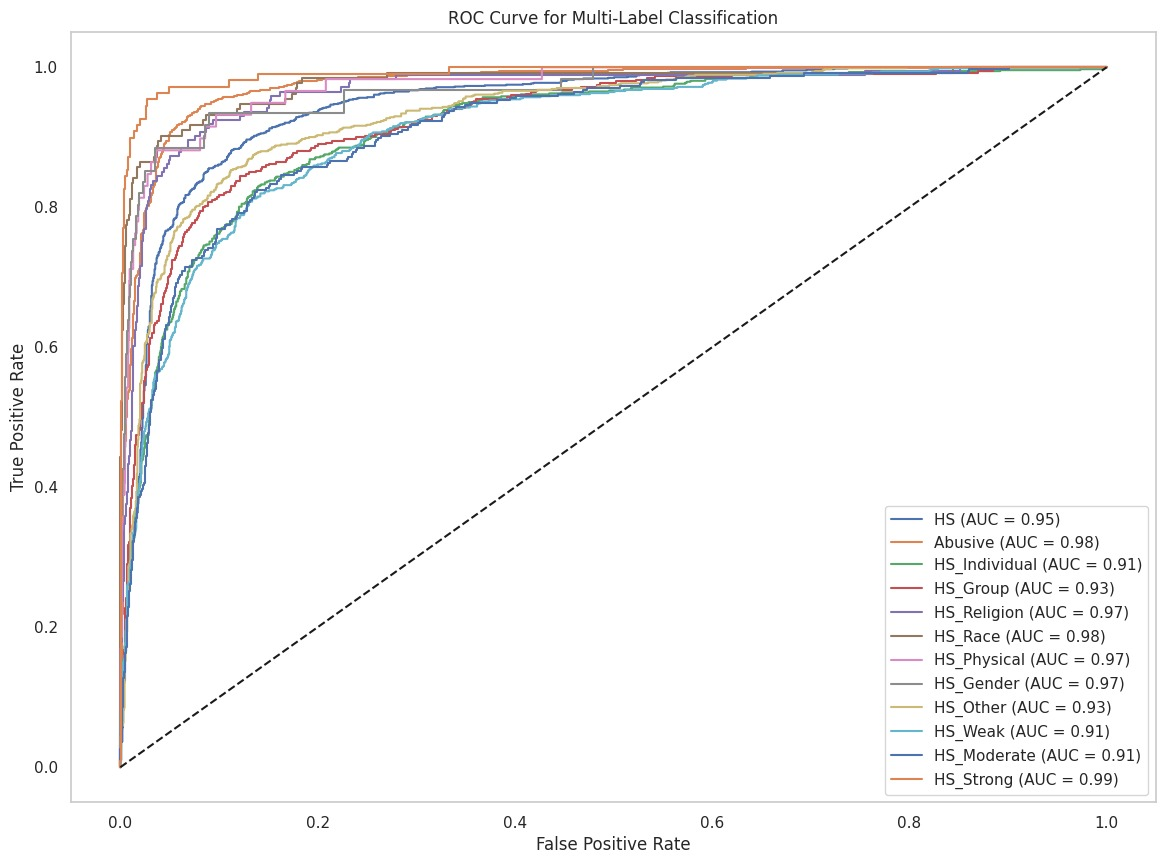
\includegraphics[width=0.5\linewidth]{Image/grafik.jpg}
    \label{fig:enter-label}

Nilai ROC-AUC ini menunjukkan bahwa model memiliki kemampuan cukup baik untuk membedakan antara kelas positif dan negatif, dengan hasil tertinggi pada label HSStrong (AUC 0.991), menunjukkan hampir sempurna dalam mendeteksi komentar yang termasuk dalam kategori ini.
\end{figure}

\begin{figure}[h]
Nilai ROC-AUC ini menunjukkan bahwa model memiliki kemampuan cukup baik untuk membedakan antara kelas positif dan negatif, dengan hasil tertinggi pada label HSStrong (AUC 0.991), menunjukkan hampir sempurna dalam mendeteksi komentar yang termasuk dalam kategori ini.
    
\end{figure}


\begin{document}

\subsection{Backend}

\section*{API Endpoint dan Respons}

\section*{API Endpoint Login}

Endpoint : POST \texttt{https://api.safespeak.info/login}

Input:
\begin{verbatim}
        {
          "username": "admin",
          "password": "******"
        }
\end{verbatim}

Output:
\begin{verbatim}
        {
          "access_token": "eyJhbGciOiJIUzI1NiIsInR5cCI6IkpXVCJ9.
          
          eyJzdWIiOiJhZG1pbiIsImV4cCI6MTU3MzNk0N30. 
          
          U1NACGtCP3bPqefsQ5oBtsOuKdddeIHE4-PvzI",
          "token_type": "bearer"
        }
\end{verbatim}

\section*{API Endpoint History}

Endpoint : GET \texttt{https://api.safespeak.info/history}

Input:
\begin{verbatim}
        {
          ...
        }
\end{verbatim}

Output:
\begin{verbatim}
        {
          "Komentar": "Anjing peliharaan kamu sangat lucu",
          "Sentimen": "Positive",
          "HS": false,
          "Abusive": false,
          "HS_Individual": false,
          "HS_Group": false,
          "HS_Religion": false,
          "HS_Race": false,
          "HS_Physical": false,
          "HS_Gender": false,
          "HS_Other": false,
          "HS_Weak": false,
          "HS_Moderate": false,
          "HS_Strong": false,
          "Id": 21
        }
\end{verbatim}

\section*{API Endpoint Predict}

Endpoint : POST \texttt{https://api.safespeak.info/predict}

Input:
\begin{verbatim}
        {
          "comment": "sialan kamu!"
        }
\end{verbatim}

Output:
\begin{verbatim}
        {
          "message": "1,1,1,0,0,0,0,0,1,1,0,0",
          "isPositive": false
        }
\end{verbatim}


\subsection{Frontend}

\begin{figure}[h]
    \centering
    \includegraphics[width=0.5\linewidth]{Image/ss1.png}
    \hspace*{15em} % Menambahkan indentasi/tab pada caption
    \caption*{\hspace*{8em}Gambar 1 Tampilan Home}
    \label{fig:enter-label}
\end{figure}

\begin{figure}[h]
    \centering
    \includegraphics[width=0.5\linewidth]{Image/ss2.png}
     \hspace*{15em}
    \caption*{\hspace*{8em}Gambar 2 Tampilan Klasifikasi}
    \label{fig:enter-label}
\end{figure}

\begin{figure}[h]
    \centering
    \includegraphics[width=0.5\linewidth]{Image/ss4.png}
     \hspace*{15em}
    \caption*{\hspace*{8em}Gambar 3 Tampilan Input Komentar}
    \label{fig:enter-label}
\end{figure}

\begin{figure}[h]
    \centering
    \includegraphics[width=0.5\linewidth]{Image/ss5.png}
    \hspace*{15em}
    \caption*{\hspace*{4em}Gambar 4 Tampilan Hasil Klasifikasi Komentar Negatif}
     \hspace*{15em}
    \label{fig:enter-label}
\end{figure}

\begin{figure}[h]
    \centering
    \includegraphics[width=0.5\linewidth]{Image/ss6.png}
    \hspace*{15em}
    \caption*{\hspace*{4em}Gambar 5 Tampilan Hasil Deteksi Positif}
     \hspace*{15em}
    \label{fig:enter-label}
\end{figure}

\begin{figure}[h]
    \centering
    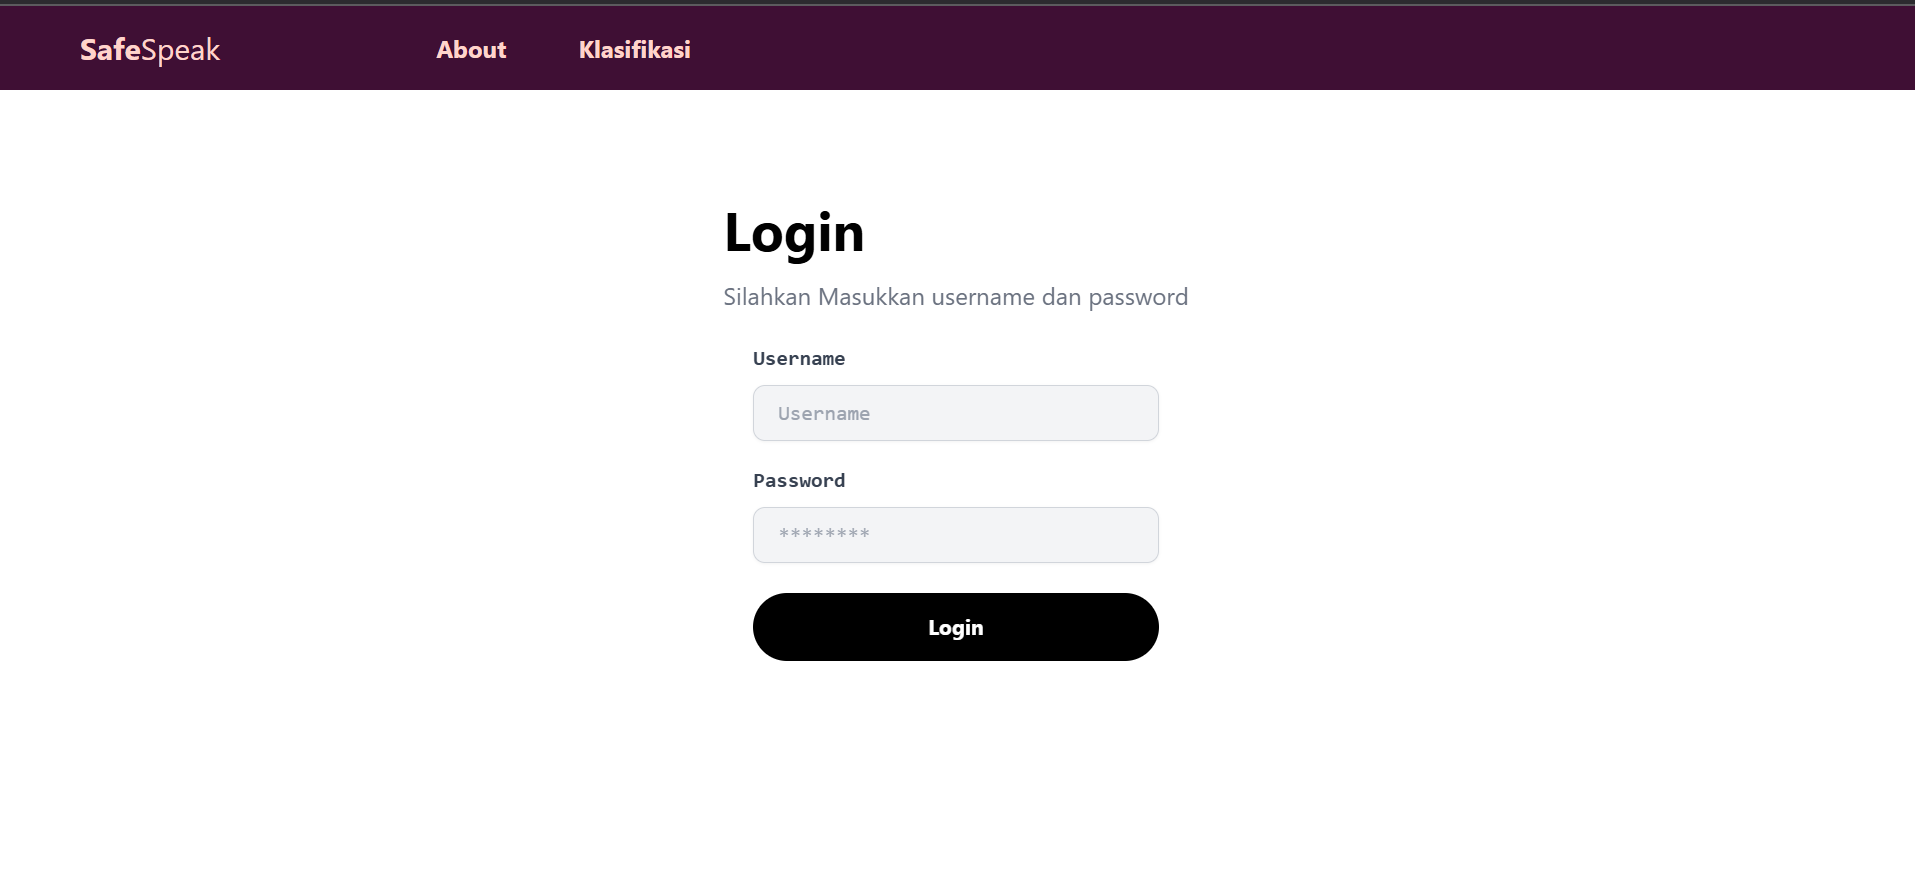
\includegraphics[width=0.5\linewidth]{Image/ss7.png}
     \hspace*{15em}
    \caption*{\hspace*{4em}Gambar 6 Tampilan Login Pada Admin}
    \label{fig:enter-label}
\end{figure}

\begin{figure}[h]
    \centering
    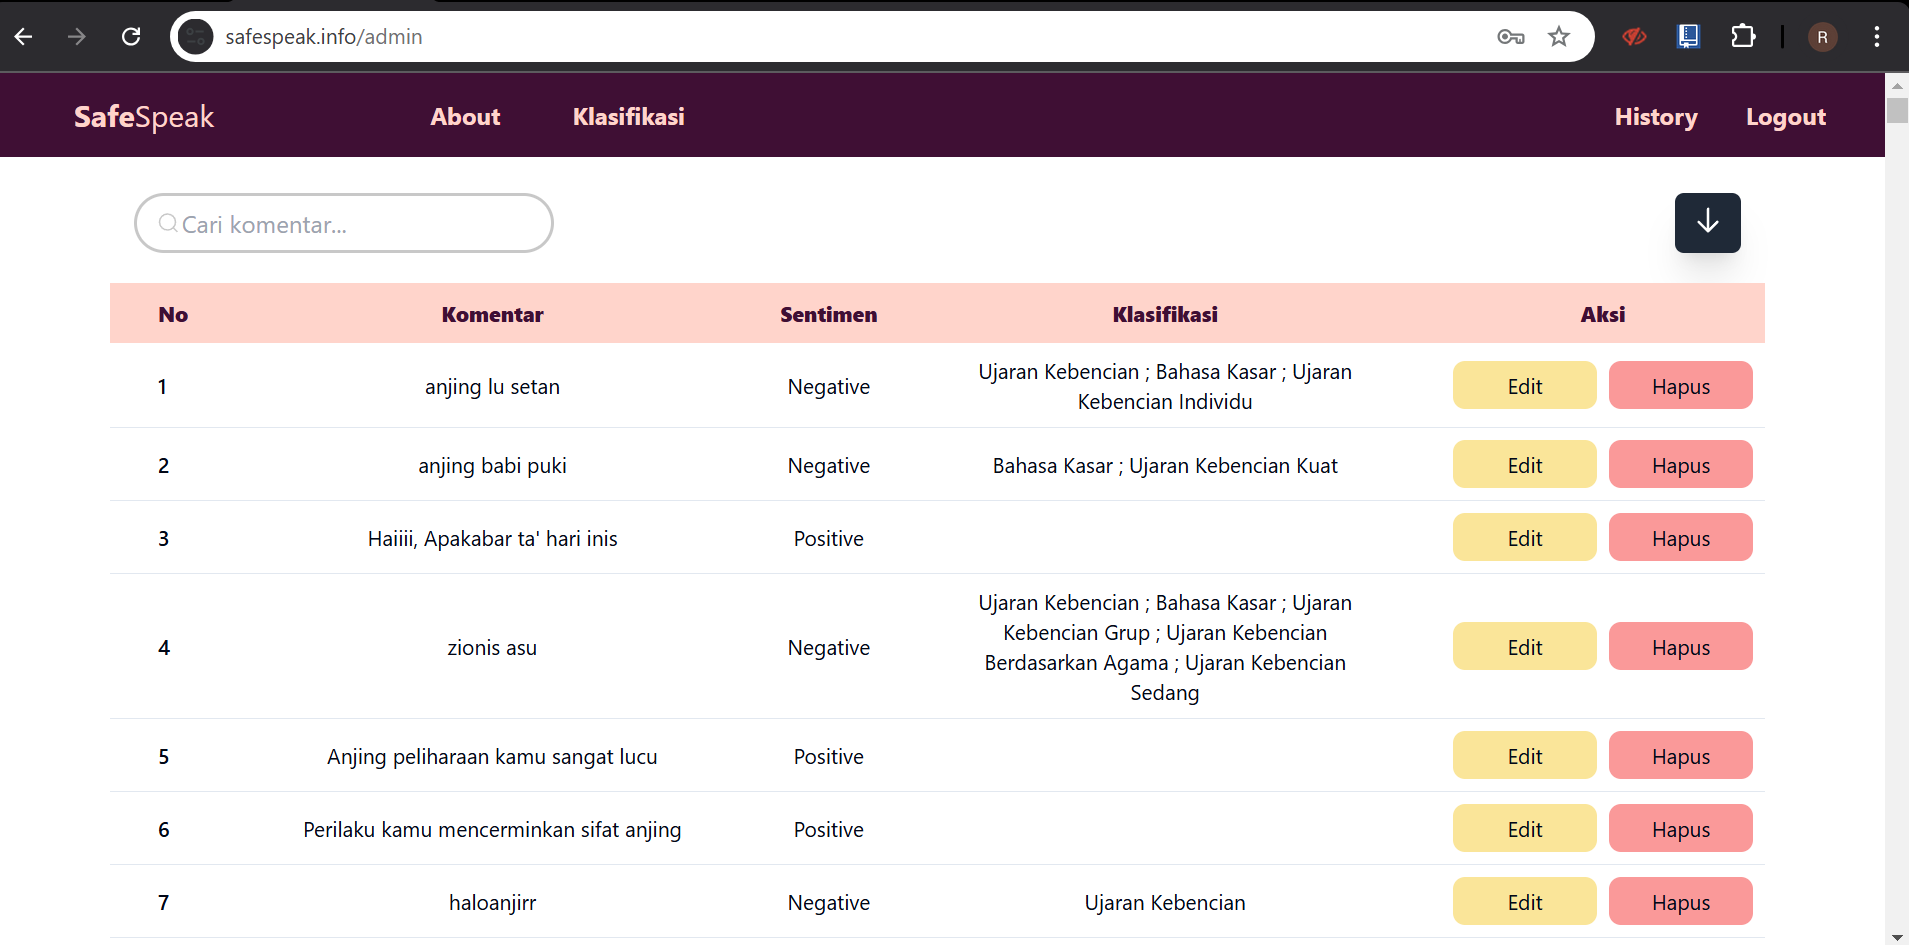
\includegraphics[width=0.5\linewidth]{Image/ss8.png}
     \hspace*{15em}
    \caption*{\hspace*{5em}Gambar 7 Tampilan History Pada Admin}
    \label{fig:enter-label}
\end{figure}

\end{document}
\end{document}

\begin{document}

\subsection{Backend}

\section*{API Endpoint dan Respons}

\section*{API Endpoint Login}

Endpoint : POST \texttt{https://api.safespeak.info/login}

Input:
\begin{verbatim}
        {
          "username": "admin",
          "password": "******"
        }
\end{verbatim}

Output:
\begin{verbatim}
        {
          "access_token": "eyJhbGciOiJIUzI1NiIsInR5cCI6IkpXVCJ9.
          
          eyJzdWIiOiJhZG1pbiIsImV4cCI6MTU3MzNk0N30. 
          
          U1NACGtCP3bPqefsQ5oBtsOuKdddeIHE4-PvzI",
          "token_type": "bearer"
        }
\end{verbatim}

\section*{API Endpoint History}

Endpoint : GET \texttt{https://api.safespeak.info/history}

Input:
\begin{verbatim}
        {
          ...
        }
\end{verbatim}

Output:
\begin{verbatim}
        {
          "Komentar": "Anjing peliharaan kamu sangat lucu",
          "Sentimen": "Positive",
          "HS": false,
          "Abusive": false,
          "HS_Individual": false,
          "HS_Group": false,
          "HS_Religion": false,
          "HS_Race": false,
          "HS_Physical": false,
          "HS_Gender": false,
          "HS_Other": false,
          "HS_Weak": false,
          "HS_Moderate": false,
          "HS_Strong": false,
          "Id": 21
        }
\end{verbatim}

\section*{API Endpoint Predict}

Endpoint : POST \texttt{https://api.safespeak.info/predict}

Input:
\begin{verbatim}
        {
          "comment": "sialan kamu!"
        }
\end{verbatim}

Output:
\begin{verbatim}
        {
          "message": "1,1,1,0,0,0,0,0,1,1,0,0",
          "isPositive": false
        }
\end{verbatim}


\subsection{Frontend}

\begin{figure}[h]
    \centering
    \includegraphics[width=0.5\linewidth]{Image/ss1.png}
    \hspace*{15em} % Menambahkan indentasi/tab pada caption
    \caption*{\hspace*{8em}Gambar 1 Tampilan Home}
    \label{fig:enter-label}
\end{figure}

\begin{figure}[h]
    \centering
    \includegraphics[width=0.5\linewidth]{Image/ss2.png}
     \hspace*{15em}
    \caption*{\hspace*{8em}Gambar 2 Tampilan Klasifikasi}
    \label{fig:enter-label}
\end{figure}

\begin{figure}[h]
    \centering
    \includegraphics[width=0.5\linewidth]{Image/ss4.png}
     \hspace*{15em}
    \caption*{\hspace*{8em}Gambar 3 Tampilan Input Komentar}
    \label{fig:enter-label}
\end{figure}

\begin{figure}[h]
    \centering
    \includegraphics[width=0.5\linewidth]{Image/ss5.png}
    \hspace*{15em}
    \caption*{\hspace*{4em}Gambar 4 Tampilan Hasil Klasifikasi Komentar Negatif}
     \hspace*{15em}
    \label{fig:enter-label}
\end{figure}

\begin{figure}[h]
    \centering
    \includegraphics[width=0.5\linewidth]{Image/ss6.png}
    \hspace*{15em}
    \caption*{\hspace*{4em}Gambar 5 Tampilan Hasil Deteksi Positif}
     \hspace*{15em}
    \label{fig:enter-label}
\end{figure}

\begin{figure}[h]
    \centering
    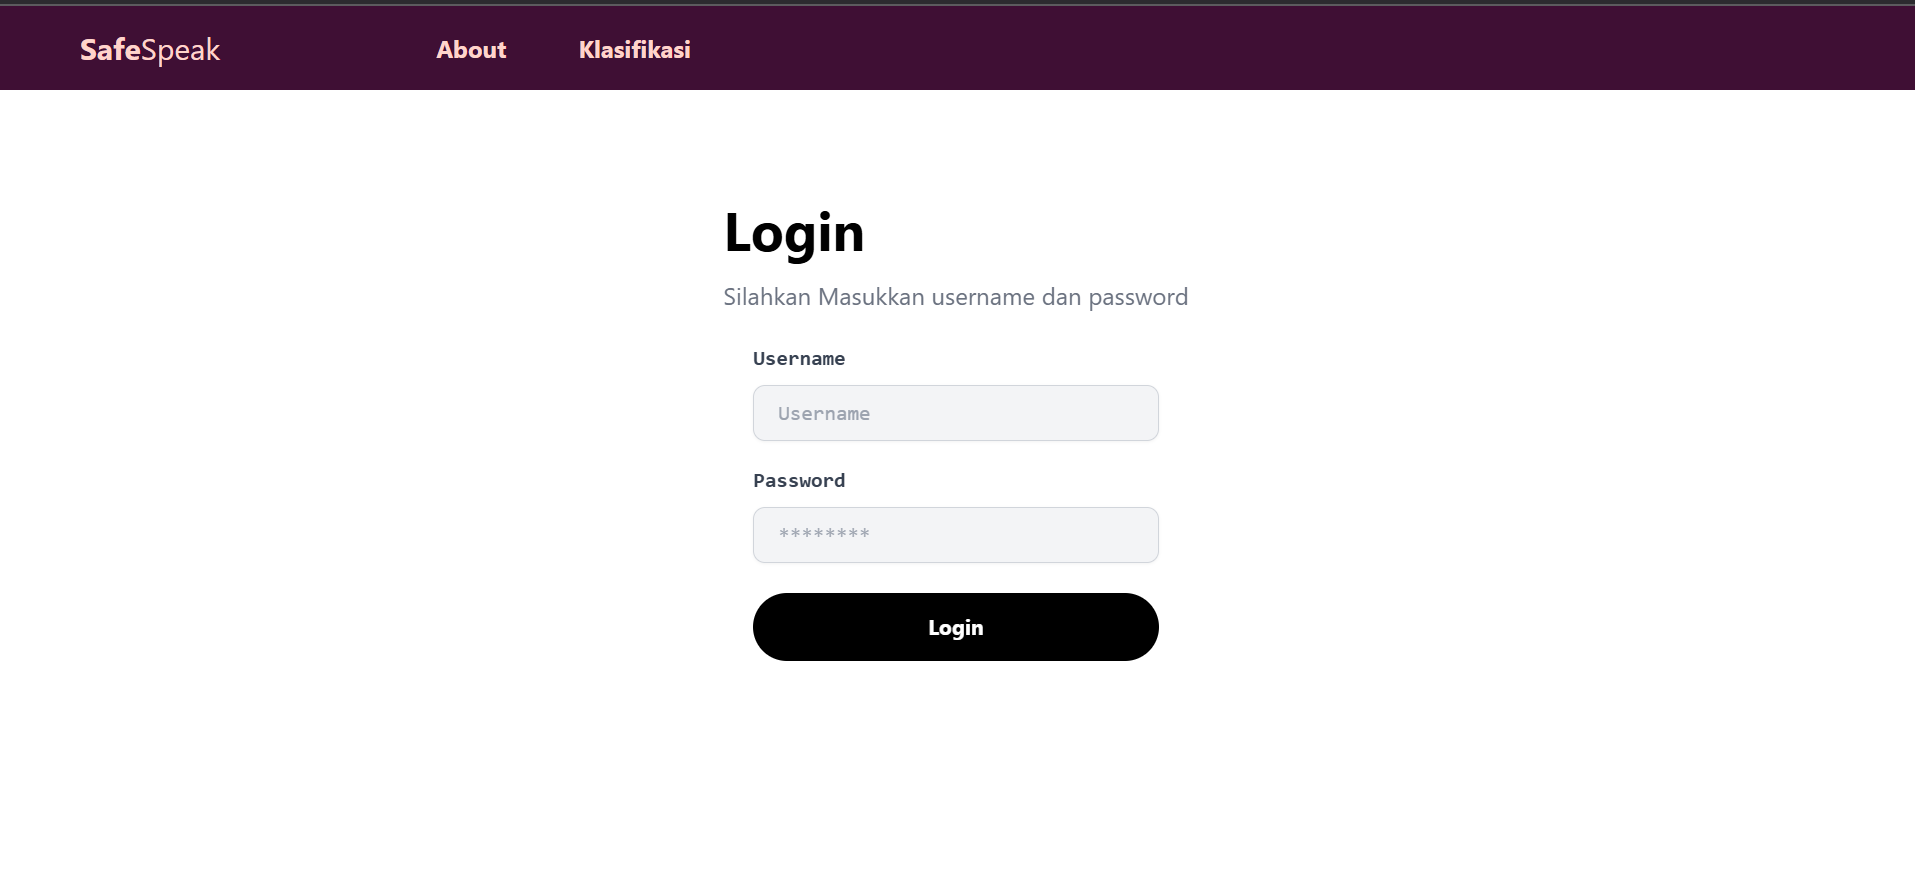
\includegraphics[width=0.5\linewidth]{Image/ss7.png}
     \hspace*{15em}
    \caption*{\hspace*{4em}Gambar 6 Tampilan Login Pada Admin}
    \label{fig:enter-label}
\end{figure}

\begin{figure}[h]
    \centering
    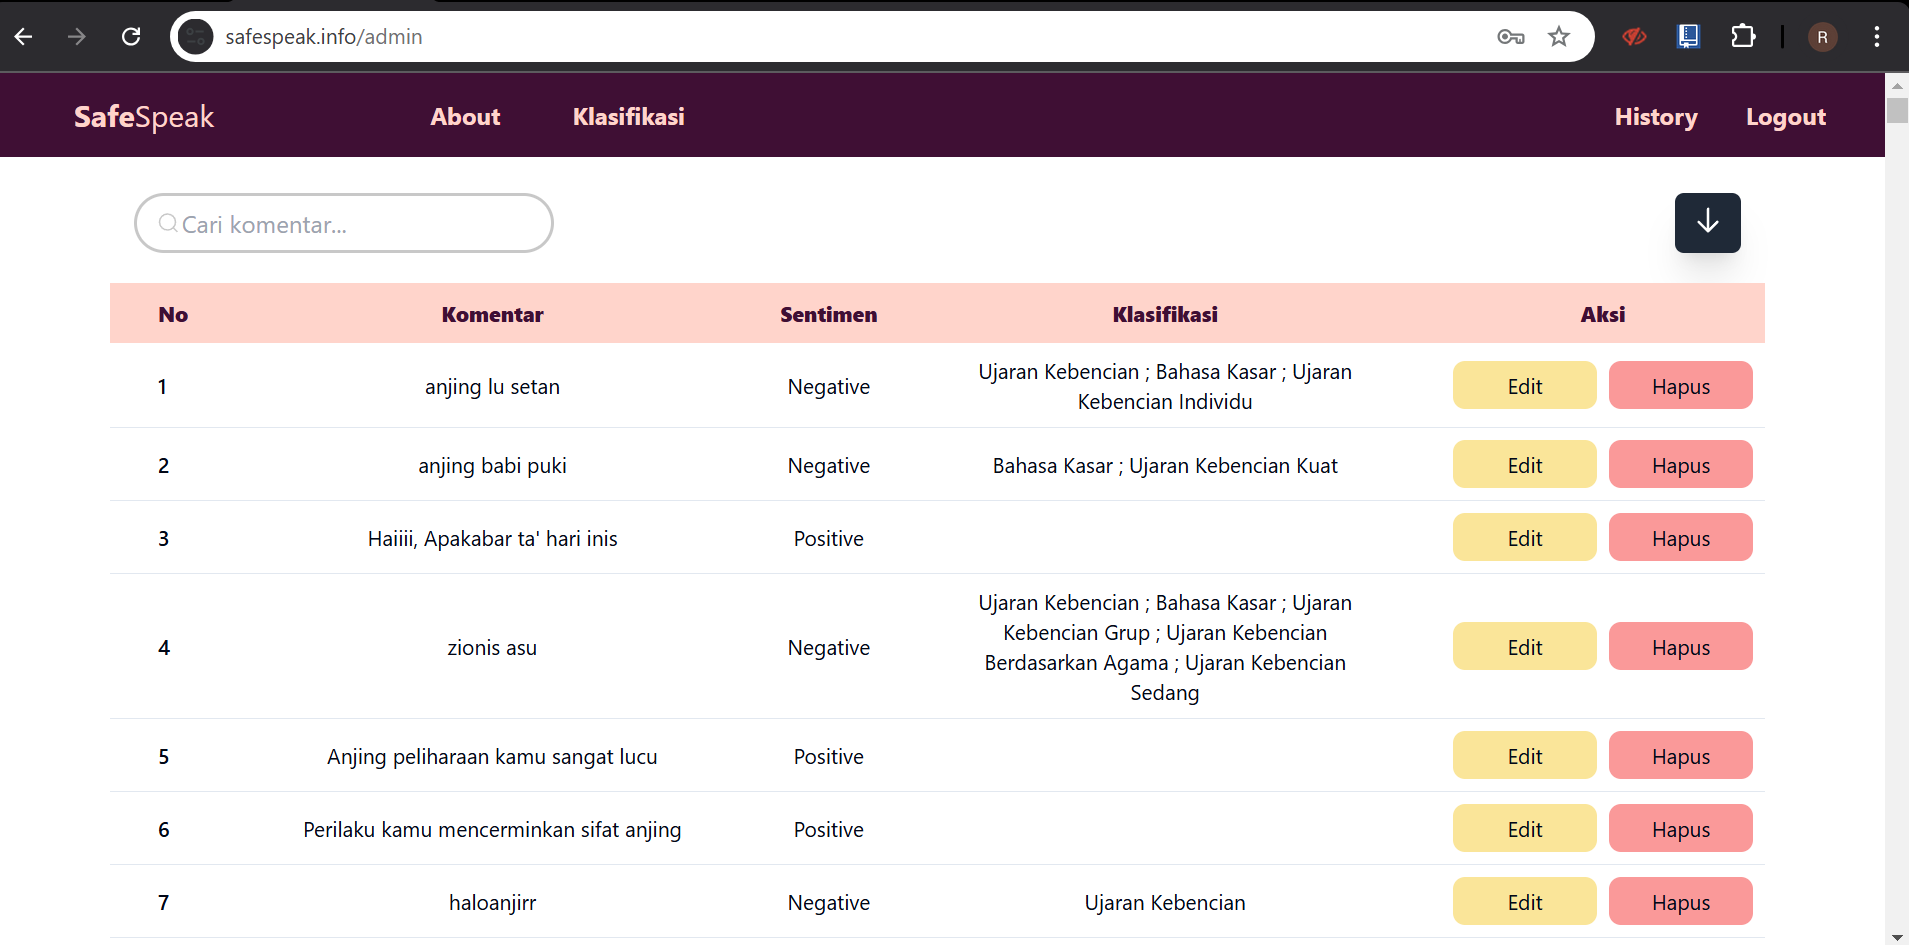
\includegraphics[width=0.5\linewidth]{Image/ss8.png}
     \hspace*{15em}
    \caption*{\hspace*{5em}Gambar 7 Tampilan History Pada Admin}
    \label{fig:enter-label}
\end{figure}

\end{document}

% \begin{document}
% \subsection{Backend}

% \section*{API Endpoint dan Respons}

% \section*{API Endpoint Login}

% Endpoint : POST \texttt{https://api.safespeak.info/login}

% Input    :
% \begin{lstlisting}
% \{
%   "username": "admin",
%   "password": "******"
% \}
% \end{lstlisting}

% Output   :
% \begin{lstlisting}
% \{
%   "access_token": "eyJhbGciOiJIUzI1NiIsInR5cCI6IkpXVCJ9.
  
%   eyJzdWIiOiJhZG1pbiIsImV4cCI6MTU3MzNk0N30.
  
%   U1NACGtCP3bPqefsQ5oBtsOuKdddeIHE4-PvzI",
  
%   "token_type": "bearer"
% \}
% \end{lstlisting}

% \section*{API Endpoint History}

% Endpoint : GET \texttt{https://api.safespeak.info/history}

% Input    :
% \begin{lstlisting}
% \{
%   ...
% \}
% \end{lstlisting}

% Output   :
% \begin{lstlisting}
% \{
%   "Komentar": "Anjing peliharaan kamu sangat lucu",
%   "Sentimen": "Positive",
  
%   "HS": false,
%   "Abusive": false,
%   "HS_Individual": false,
%   "HS_Group": false,
  
%   "HS_Religion": false,
%   "HS_Race": false,
%   "HS_Physical": false,
%   "HS_Gender": false,
  
%   "HS_Other": false,
%   "HS_Weak": false,
%   "HS_Moderate": false,
%   "HS_Strong": false,
  
%   "Id": 21
% \}
% \end{lstlisting}

% \section*{API Endpoint Predict}

% Endpoint : POST \texttt{https://api.safespeak.info/predict}

% Input    :
% \begin{lstlisting}
% \{
%   "comment": "sialan kamu!"
% \}
% \end{lstlisting}

% Output   :
% \begin{lstlisting}
% \{
%   "message": "1,
%   1,
%   1,
%   0,
%   0,
%   0,
%   0,
%   0,
%   1,
%   1,
%   0,
%   0",
%   "isPositive": false
% \}
% \end{lstlisting}

% \subsection{Frontend}
% \begin{figure}
%     \centering
%     \includegraphics[width=0.5\linewidth]{ss1.png}
%     \caption*{Gambar 1 Tampilan Home}
%     \label{fig:enter-label}
% \end{figure}

% \begin{figure}
%     \centering
%     \includegraphics[width=0.5\linewidth]{ss2.png}
%     \caption*{Gambar 2 Tampilan Klasifikasi}
%     \label{fig:enter-label}
% \end{figure}

% \begin{figure}
%     \centering
%     \includegraphics[width=0.5\linewidth]{ss3.png}
%     \caption*{Gambar 3 Tampilan}
%     \label{fig:enter-label}
% \end{figure}

% \begin{figure}
%     \centering
%     \includegraphics[width=0.5\linewidth]{ss4.png}
%     \caption*{Gambar 4 Tampilan Input Komentar}
%     \label{fig:enter-label}
% \end{figure}

% \begin{figure}
%     \centering
%     \includegraphics[width=0.5\linewidth]{ss5.png}
%     \caption*{Gambar 5 Tampilan Hasil Klasifikasi Komentar Negatif}
%     \label{fig:enter-label}
% \end{figure}

% \begin{figure}
%     \centering
%     \includegraphics[width=0.5\linewidth]{ss6.png}
%     \caption*{Gambar 6 Tampilan Hasil Deteksi Positif}
%     \label{fig:enter-label}
% \end{figure}

% \end{document}



% \begin{document}
% \subsection{Frontend}
% \begin{figure}
%     \centering
%     \includegraphics[width=0.5\linewidth]{ss1.png}
%     \caption*{Gambar 1 Tampilan Home}
%     \label{fig:enter-label}
% \end{figure}

% \begin{figure}
%     \centering
%     \includegraphics[width=0.5\linewidth]{ss2.png}
%     \caption*{Gambar 2 Tampilan Klasifikasi}
%     \label{fig:enter-label}
% \end{figure}

% \begin{figure}
%     \centering
%     \includegraphics[width=0.5\linewidth]{ss3.png}
%     \caption*{Gambar 3 Tampilan}
%     \label{fig:enter-label}
% \end{figure}

% \begin{figure}
%     \centering
%     \includegraphics[width=0.5\linewidth]{ss4.png}
%     \caption*{Gambar 4 Tampilan Input Komentar}
%     \label{fig:enter-label}
% \end{figure}

% \begin{figure}
%     \centering
%     \includegraphics[width=0.5\linewidth]{ss5.png}
%     \caption*{Gambar 5 Tampilan Hasil Klasifikasi Komentar Negatif}
%     \label{fig:enter-label}
% \end{figure}

% \begin{figure}
%     \centering
%     \includegraphics[width=0.5\linewidth]{ss6.png}
%     \caption*{Gambar 6 Tampilan Hasil Deteksi Positif}
%     \label{fig:enter-label}
% \end{figure}
% \end{document}


% \end{document}

% \begin{table}[H]
% \caption{This is another table.\label{tab2}}
% \begin{tabularx}{\textwidth}{CCCC}
% \toprule
% \textbf{Title 1}	& \textbf{Title 2}	& \textbf{Title 3}     & \textbf{Title 4}\\
% \midrule
% Entry 1	& Data	& Data	& Data\\
% Entry 2	& Data	& Data	& Data\\
% \bottomrule
% \end{tabularx}
% \end{table}

% \begin{equation}
% a = b + c + d + e + f + g + h + i + j + k + l + m + n + o + p + q + r + s + t + u + v + w + x + y + z
% \end{equation}

